\chapter{Implementation}

\section{Introduction}
This chapter details the implementation of the MASDR platform. The description has been divided into software and hardware for clarity.

\section{Software Implementation}
The software for the MASDR system was written in C++ and can be found in the appendix to this report. Documentation was done with doxygen, allowing for dynamic updates to the docs whenever changes were made. The final version of the documentation can also be found in the appendix. Additionally, some scripts were written to assist in other aspects of the project.
\subsection{C++ vs GNU Radio}
During the design phase, there was discussion over whether to use GNU radio or C++ for the MASDR application. GNU radio would allow for more complex signal processing patterns to be constructed more easily in comparison to C++, but would increase the overhead on development and potentially at runtime as well. Using C++, the application would have to be coded entirely from scratch, interfacing with the USRP Hardware Driver (UHD) libraries, but would have much lower overhead. Based on the skills of the team members, as well as the desire for the application to be as low power and simple as possible, C++ was chosen for the application.
\subsection{Application Structure} \textbf{NEEDS TO BE UPDATED}
The MASDR Application is structured as a central C++ class with a few additional utility functions external to the class. The class contains methods for initialization, sampling, processing, and transmission among others. Certain services, notably updating the GPS and taking in samples, are performed in separate threads to allow for the parallelization of tasks. In the application’s main loop, an instance of the MASDR class updates its status and begins or changes its task based on the new status. Status is composed of both physical status, namely location, and software status, representing the current processing state. The physical status structure includes a member variable for heading, although this is unused in the current version of the platform. The processing state is an enumerated type with values PROCESS, TRANSMIT, and IDLE. The state of the device determines what the processor will be doing. During operation, the application will flow from state to state as described in the state transition diagram in Figure \ref{fig:state_diagram}. \par
\begin{figure}[ht]
\centering
\includegraphics[width=0.70\textwidth]{img/masdr_state_diagram.png}
\caption{MASDR State Diagram. Software states change according to the graph described in the image.}
\label{fig:state_diagram}
\end{figure}
The onboard software is the majority of the project, however there are other essential pieces. On the ground station side, a GNU radio receiver receives and decodes all transmissions from the aerial platform. Additionally, a mapping tool was created to calculate the approximate distance to signals and draw circles on a map to visually locate signals. The mapping tool consists of a python script that performs the distance calculations and populates a javascript list of gps locations and distances. The javascript calls into the Google Maps API to display the distance rings on a map. Finally, a python script was written to command the drone to autonomously spin 360 degrees.
\subsection{Sampling Procedure} \label{impl:rotate}
While the original plan was for the sampling routine to be mainly driven by the motion of the platform, a lack of precision and accuracy in the GPS readings rendered this nearly impossible. Therefore, the SDR was configured to constantly take samples, with control originating from a separate processing thread from the main thread. The use of threads allows for shared data throughout the program, which is used to share the  buffer of samples with the main thread. \par
In order to avoid any shared data bugs, the sampling routine fills a buffer of blocks one at a time, eventually overwriting the oldest block to record each new block. At the beginning of the processing routine, a copy of the most recent half of the sample blocks is made. This makes it impossible for the sampling thread to overwrite a block of samples that the processing thread is using. \par
There is a defined motion pattern that the quadcopter should follow in order achieve correct results. At a constant altitude, the quadcopter should travel to a series of points, stopping and rotating 360 degrees at each point. The constant altitude will allow for more accurate localization of signals based on RSSI distance.
\subsection{Onboard Processing}
The samples taken by the SDR are then processed to extract useful information. Given that the MASDR system is designed to be low power, a delineation between onboard processing and processing at the ground station was created. The UP board’s processor is fairly capable, allowing the initial steps of the signal processing to be done onboard. A more indepth description of the processing done onboard the MASDR platform can be found in Methodology section \ref{methods:processing}. The information is processed as much as possible onboard to reduce the size and duration of the transmissions to the ground station. The initial samples are also stored on a flash drive onboard so that post processing can be done on the raw data. \par
To detect the existence of a signal, an OFDM receiver in the MASDR application looks for beacon signals in the sampled data, block by block. The RSS of a beacon signal is recorded with its corresponding location, the location the drone was at when the block of samples were taken. This mapping is then transmitted down to the ground station for further processing.
\subsection{Data Transmission}
The MASDR platform is designed to transmit data between processing blocks of samples. The transmission protocol consists of two types of messages: a header packet, and a data packet. The header packet is the first packet sent after processing data; it contains a transmission ID, the location of the sampling block, and the number of following data transmissions. The data packet consists of a transmission ID which corresponds to its header packet, a heading, and a signal strength for beacon signals. Again, the heading is unused in the current version of the platform, but a future version could make use of the field.

\section{Hardware Implementation}
The hardware for the MASDR system consists of the components used and the mounting system employed to attach it all to the drone. Using the 3DR Solo’s development guide as a reference, the mounting system was designed to hold all the components securely to the drone. By using the official mounting points on the drone, the hardware was made as robust and efficient as possible.
\subsection{Mounting on Drone} \label{Mounting}
In order for the hardware to be mounted properly, the MASDR system was mounted onto the drone platform by using the Solo’s preexisting hardware mount. To do this, the 3DR Solo’s developer's guide was used to determine the dimensions of the mounting screws so that the mounting platform was able to be easily screwed onto the 3DR solo. The mounting system connects to the bottom of the 3dr solo with four M2 screws that are spaced in a 63mm x 41mm rectangular pattern as seen in Figure \ref{fig:solo_mount}.
\begin{figure}[ht]
\centering
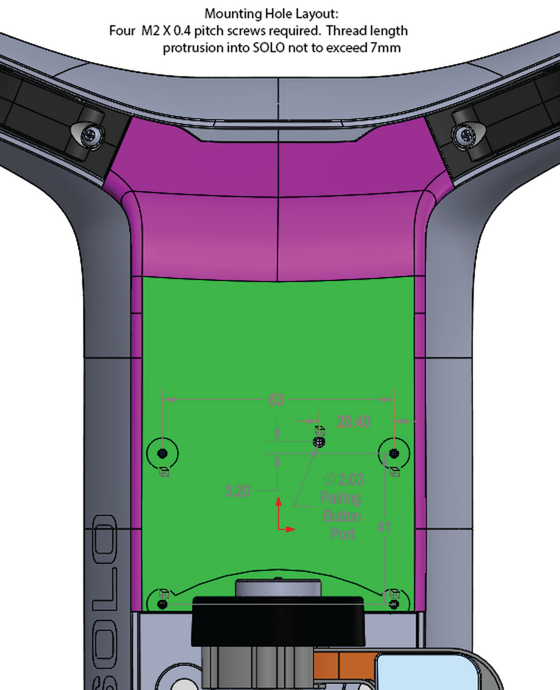
\includegraphics[width=0.70\textwidth]{img/solo_mount_points.png}
\caption{3DR Solo Mounting Points}
\label{fig:solo_mount}
\end{figure} \par
The mounting system consisted of two pieces of wood lasercut with a lightening and mounting pattern. The pieces were attached with 3 inch standoffs, allowing room for the UP board, B-200 mini, tranformer, and battery to be mounted and connected together. A picture of the assembled mounting system can be seen in Figure \ref{fig:overhead_of_box} and Figure \ref{fig:box_usb_view}.

\subsection{Power Conversion}
In order to ensure that the MASDR platform is powered for the entire flight, a battery was needed that could hold as much energy as possible while not adding too much weight to the drone’s payload. In addition to this, the battery needed be able to supply as much current as the hardware could draw. This became an issue for finding a suitable 5V battery that would support a maximum current draw of 4 Amps. Instead of a 5 volt battery, a 12 volt battery was used, and a DC-DC converter was used to match the 5V 4A requirement. The chosen battery was an 11.1 volt lithium-polymer battery weighing 66 grams. It was then connected to a DROK DC voltage converter that both transformed and regulated the voltage to 5V. By down converting the voltage from the battery, the system is able to draw more current from the battery than what is usually supported by a 5 volt battery.
\subsection{Networking Card Swap}
The 3DR Solo’s default wireless card communicates to the controller using the 2.4 GHz band. This interferes with sensing and locating signals on the 2.4 GHz band. In order to avoid this issue, the 2.4 GHz network card of the 3DR Solo was replaced with a dual band 2.4 GHZ and 5 GHz network card. Unfortunately, even with the new wireless card, the controller and drone were unable to communicate on the 5 GHz band. It is suspected that this is due to incompatible antennas.




